%%%%%%%%%%%%%%%%%%%
\clearpage

\section{Dstar}
\subsection{Data set abs experiment cuts}
We used Au+Au 200 GeV data collected in RHIC Run 14 and Run 16 utlizing HFT detector. 
o0o0o0o0o0o0o0o0o0\\
this is a test if git works \\
o0o0o0o0o0o0o0o0o0o\\
\subsubsection{Event and track level cut}
For both Run 14 and Run 16 dataset: \\
$|Vz|<6~cm$ \\
$|Vz_{vpd}-Vz_{TPC}|< 3~cm$ \\
$|Vx,Vy,Vz|_{at~least~one}> 10^{-5}~cm$\\
$|\sqrt{Vx^{2}+Vy^{2}}|< 2~cm$ 
\par
Track quality cut:\\
$nHitsFit > 20$\\
$|eta|<1$\\
For $D^{0}$ daughters:\\
 global tracks and require have at least one hit on HFT\\
 global $p_{T}>$0.3GeV for Run 14 and $>$0.6 GeV for Run 16\\
For soft pion:\\
 global tracks and $|gDCA|<$  3cm, global $p_{T}>$ 0.15 GeV
\subsection{$D^{*+}$ reconstruction}
	$D^{*+}$ is reconstruct by $D^{*+}\rightarrow D^{0}\pi^{+})$(B.R.=67.7\%), $D^{0}\rightarrow K^{-}\pi^{+}$(B.R.=3.89\%) and its charge conjugate channel. The Fig. \ref{fig:decayTopo} shows $D^{*+}$ decay topology. We first reconstruct $D^{0}$ ultilizing HFT detector, and then pair the $D^{0}$ candidate with a soft pion. As this pion usually have a very soft transvrese momentum (about 1/11 with recpect to $D^{*}$), we apply a very loose cut. We choose the global tracks without requiring HFT hits(see in the track level cut). For the $D^{0}$ candidate mass window cut, to ensure 100\% efficiency on this cut, the mass windows is chosen within 3.5 sigma depending on the $D^{0}$ $p_{T}$.  
	\par
	For the $D^{0}$ daughters' PID cut:\\
	K: $|nSigma|<2$; if TOF available, $|\frac{1}{\beta_{exp}}-\frac{1}{\beta_{th}}|<0.03$, otherwise TPC only.
\\
	$\pi$: $|nSigma|<2$; if TOF available, $|\frac{1}{\beta_{exp}}-\frac{1}{\beta_{th}}|<0.02$, otherwise TPC only.
	\par
	For the $\pi_{soft}$, as at the very low $p_{T}$ ($p_{T}<0.3 GeV$), the calibration of the TOF has some shift so we choose a $p_{T}$ dependent $1/\beta$ cut.
	
	\begin{figure}[h!]
		\centering
		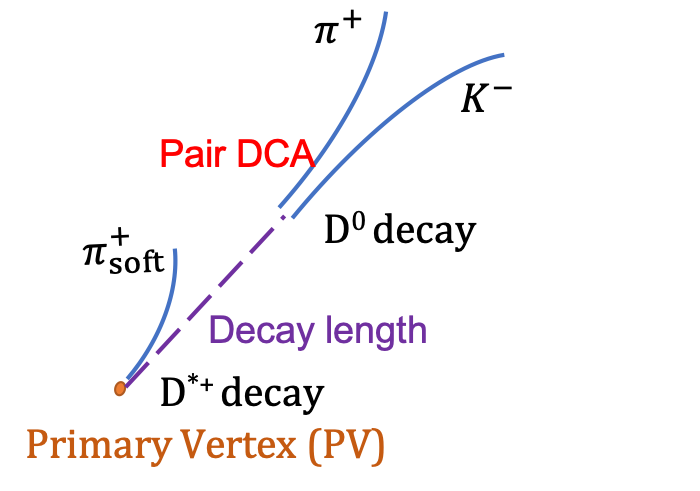
\includegraphics[scale=0.6]{dstarplots/decayTopo.png}
		\caption{$D^{*+}~decay~topology$}
		\label{fig:decayTopo}
	\end{figure}
	
		\begin{figure}[h!]
		\centering
		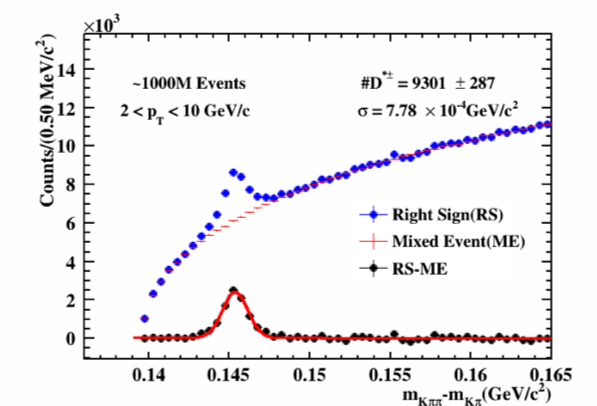
\includegraphics[scale=1]{dstarplots/sig16.png}
		\caption{$D^{*\pm}$ signal in Run 16}
		\label{fig:sig16}
	\end{figure}

\subsection{Efficiency correction}
	The basic precedure is:
	\begin{enumerate}
    \item Extract $D^{0}$ daughter particle $K/\pi$ PID efficincy and TPC tracking efficiency, momemtum resolution, DCA resolution and HFT matching efficiency, and then running the fast simulation package to extract the $D^{0}$ reconstruction efficiency, the momemtum resolution of the $D^{0}$ can be also extracted through this procedure.
		\item Extract $\pi_{soft}$ TPC tracking and PID efficiency;
    \item Decay the $D^{*+}$ to $D^{0}\pi^{+}$ by pythia, and then apply the $\pi_{soft}$ PID/TPC tracking efficiency and $D^{0}$ reconstruction efficiency gotton from the above procedure. The acceptance cuts such as $|\eta|<1$ are also considered. Because we choose a loose (3.5 sigma) cut on the $K\pi$ pair invariant mass when choosing the $D^{0}$ candidate, so for this cut we have 100\% efficiency. Through these procedures we are able to extract $D^{*}$ efficiency. 
	\end{enumerate}
\subsubsection{$D^{0}$ reconstruction efficiency} 
$D^{0}$ reconstruction efficiency calculation is based on the fast simulation package. 
\subsubsection{$\pi_{soft}$ TPC tracking efficiency}
We use the STAR standard embedding method to calculate the TPC tracking efficiency, which is the fraction of the tracks, that are reconstructed and pass the track quality cut, with respect to the total number of the tracks. MC tracks are embedded into the full geant4 simulation of the STAR detector. And then the MC hits are mixed with the hits from the real data to go through the track reconstruction. The TPC tracking efficiency is then defined as:
\begin{equation}
\begin{aligned}
&Eff_{TPC~tracking} = \\
& \frac{N_{reconstructed~MC~tracks}(nCommenHits>10~\&~nHitsFit>20~\&~dca<3~\&|\eta|<1)}{Number~of~total~MC~tracks}
 \end{aligned}
\end{equation}
Fig. is the $\pi_{soft}$ TPC tracking efficiency in Run 14.
\begin{figure}
	\centering
	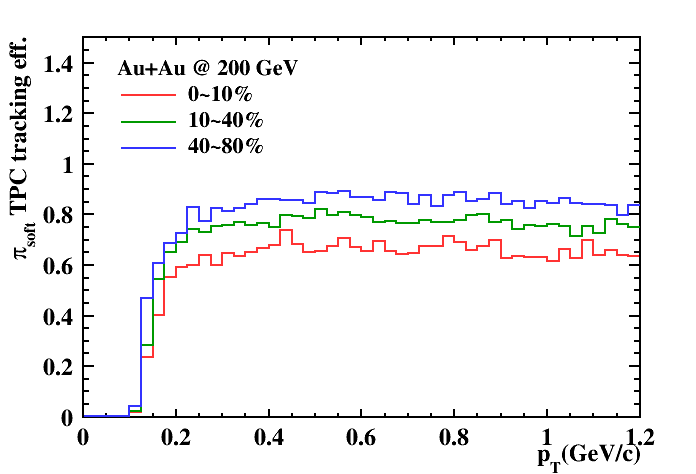
\includegraphics[scale=0.4]{dstarplots/piTPCeff.png}
	\caption{$\pi_{soft}$ TPC tracking efficiency in Run 14}
	\label{fig:piTPCeff}
\end{figure}
\subsubsection{$\pi_{soft}$ PID efficiency}
For hybrid PID, PID efficiency can be calculatecd as:
\begin{equation}
Eff_{PID} = Eff_{TPC}*Eff_{TOF}*Eff_{matching}+(1-Eff_{matching})*Eff_{TPC}
\end{equation}
$Eff_{PID}$ is the total PID efficiency, $Eff_{TPC}$ is the TPC PID efficiency, $Eff_{TOF}$ is the TOF PID efficiency, $Eff_{matching}$ is the TOF matching efficiency.
TPC PID is extract pure pion sample from $K_{s}$;
TOF PID sample is chosen from TPC PID. Because at the low $p_{T}$ if we choose the pion sample from $K_{s}$ at the low $p_{T}$, the mean value $1/\beta$ would be shift from 0 as $K_{s}$ has a very long decay length ($c\tau$~several cm). And we only care about $p_{T}<1.2GeV$ region so it doesn't matter if pion sample chosen from TPC cannot reach higher pt.
TOF match efficiency is defined as:
\begin{equation}
Eff_{TOF~matching}=\frac{N_{qualified~TPC~track}(\beta>0)}{N_{qualified~TPC~track}}
\end{equation}
\begin{figure}[h!]
	\centering
	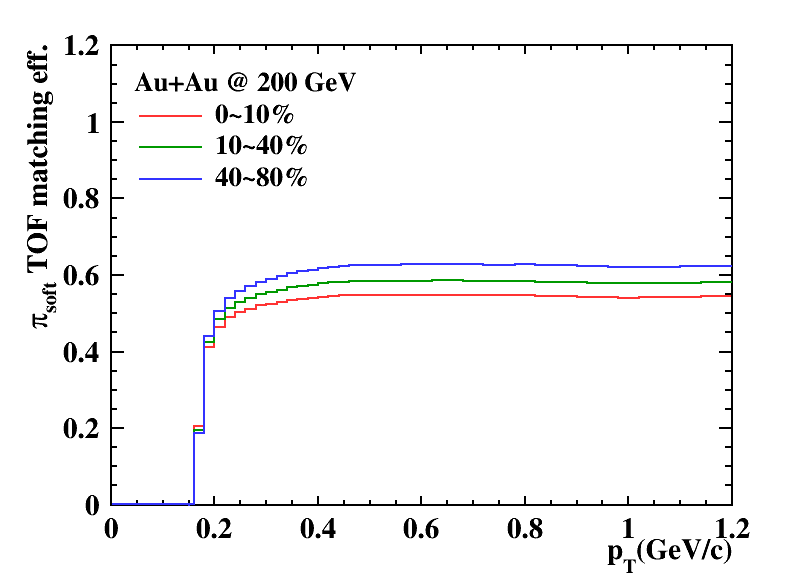
\includegraphics[scale=0.35]{dstarplots/piTofeff.png}
	\caption{$\pi_{soft}$ TOF matching efficiency in Run 14}
	\label{fig:spitof14}
\end{figure}

	\subsection{Systematic uncertainty}
	
	\subsection{Results and discusion}
	


